\documentclass{article}\usepackage[]{graphicx}\usepackage[]{color}
%% maxwidth is the original width if it is less than linewidth
%% otherwise use linewidth (to make sure the graphics do not exceed the margin)
\makeatletter
\def\maxwidth{ %
  \ifdim\Gin@nat@width>\linewidth
    \linewidth
  \else
    \Gin@nat@width
  \fi
}
\makeatother

\definecolor{fgcolor}{rgb}{0.345, 0.345, 0.345}
\newcommand{\hlnum}[1]{\textcolor[rgb]{0.686,0.059,0.569}{#1}}%
\newcommand{\hlstr}[1]{\textcolor[rgb]{0.192,0.494,0.8}{#1}}%
\newcommand{\hlcom}[1]{\textcolor[rgb]{0.678,0.584,0.686}{\textit{#1}}}%
\newcommand{\hlopt}[1]{\textcolor[rgb]{0,0,0}{#1}}%
\newcommand{\hlstd}[1]{\textcolor[rgb]{0.345,0.345,0.345}{#1}}%
\newcommand{\hlkwa}[1]{\textcolor[rgb]{0.161,0.373,0.58}{\textbf{#1}}}%
\newcommand{\hlkwb}[1]{\textcolor[rgb]{0.69,0.353,0.396}{#1}}%
\newcommand{\hlkwc}[1]{\textcolor[rgb]{0.333,0.667,0.333}{#1}}%
\newcommand{\hlkwd}[1]{\textcolor[rgb]{0.737,0.353,0.396}{\textbf{#1}}}%

\usepackage{framed}
\makeatletter
\newenvironment{kframe}{%
 \def\at@end@of@kframe{}%
 \ifinner\ifhmode%
  \def\at@end@of@kframe{\end{minipage}}%
  \begin{minipage}{\columnwidth}%
 \fi\fi%
 \def\FrameCommand##1{\hskip\@totalleftmargin \hskip-\fboxsep
 \colorbox{shadecolor}{##1}\hskip-\fboxsep
     % There is no \\@totalrightmargin, so:
     \hskip-\linewidth \hskip-\@totalleftmargin \hskip\columnwidth}%
 \MakeFramed {\advance\hsize-\width
   \@totalleftmargin\z@ \linewidth\hsize
   \@setminipage}}%
 {\par\unskip\endMakeFramed%
 \at@end@of@kframe}
\makeatother

\definecolor{shadecolor}{rgb}{.97, .97, .97}
\definecolor{messagecolor}{rgb}{0, 0, 0}
\definecolor{warningcolor}{rgb}{1, 0, 1}
\definecolor{errorcolor}{rgb}{1, 0, 0}
\newenvironment{knitrout}{}{} % an empty environment to be redefined in TeX

\usepackage{alltt}
\usepackage[letterpaper, portrait, margin=1in]{geometry}

\title{Math 680 - Assignment \#2}
\author{Kevin McGregor}
\date{October 15th, 2015}
\IfFileExists{upquote.sty}{\usepackage{upquote}}{}
\begin{document}
\maketitle

\section*{Question 1}
We're trying to minimize $\|Y-X\beta\|^2$ with respect to $\beta$.  We know that the least squares criterion is a convex function, therefore the minimum we find will be a global minimum.  The function can be rewritten as:

\begin{eqnarray*}
  \|Y-X\beta\|^2 &=& (Y-X\beta)^\top(Y-X\beta) \\
                 &=& Y^\top Y - (X\beta)^\top Y - Y^\top X\beta + (X\beta)^\top X\beta \\
                 &=& Y^\top Y - 2(X\beta)^\top Y + \beta^\top X^\top X\beta.
\end{eqnarray*}

Then, differentiating with respect to $\beta$ gives:

\begin{eqnarray*}
  \nabla_\beta \|Y-X\beta\|^2 &=& -2X^\top Y + 2X^\top X\beta.
\end{eqnarray*}

So, if we plug in the centered least squares estimate for $\beta$ into this equation, we know it will be a global minimum for the least squares criterion.

WILL COME BACK TO THIS!

\section*{Question 2}
\subsection*{(a)}
\begin{eqnarray*}
  \|\tilde{Y}-\tilde{X}\beta\|^2 + \lambda\|\beta\|^2 &=& (\tilde{Y}-\tilde{X}\beta)^\top(\tilde{Y}-\tilde{X}\beta) + \lambda\beta^\top\beta \\
                 &=& \tilde{Y}^\top\tilde{Y} - 2\beta^\top\tilde{X}^\top\tilde{Y} + \beta^\top\tilde{X}^\top\tilde{X}\beta + \lambda\beta^\top\beta \\
 \nabla f(\beta) &=& -2\tilde{X}^\top\tilde{Y} + 2\tilde{X}^\top\tilde{X}\beta + 2\lambda\beta
\end{eqnarray*}

\subsection*{(b)}
The function $f$ is quadratic in $\beta$, and the matrix in the quadratic term is $\tilde{X}^\top\tilde{X}+\lambda I$, which is positive definite.  Therefore $f$ is strictly convex.

\subsection*{(c)}
Since $f$ is strictly convex, there is only one global minimizer of $f$.

\subsection*{(d)}
See R code in ``a2\_q2d.R'' and ``centeredRidge\_func.R''

\subsection*{(e)}
The solution to ridge regression is found by setting $\nabla f(\beta)=0$, which gives us $\hat{\beta}^{(\lambda)}_{-1}=(\tilde{X}^\top\tilde{X}+\lambda I)^{-1}\tilde{X}^\top\tilde{Y}$.  So we have the expected value:

\begin{eqnarray*}
  E[\hat{\beta}^{(\lambda)}_{-1}] &=& E[(\tilde{X}^\top\tilde{X}+\lambda I)^{-1}\tilde{X}^\top\tilde{Y}] \\
            &=& (\tilde{X}^\top\tilde{X}+\lambda I)^{-1}\tilde{X}^\top E[\tilde{Y}] \\
            &=&  (\tilde{X}^\top\tilde{X}+\lambda I)^{-1}\tilde{X}^\top\tilde{X}\beta_{*-1},
\end{eqnarray*}
and the variance:

\begin{eqnarray*}
  var[\hat{\beta}^{(\lambda)}_{-1}] &=& var[(\tilde{X}^\top\tilde{X}+\lambda I)^{-1}\tilde{X}^\top\tilde{Y}] \\
            &=& [(\tilde{X}^\top\tilde{X}+\lambda I)^{-1}\tilde{X}^\top] var[\tilde{Y}] [(\tilde{X}^\top\tilde{X}+\lambda I)^{-1}\tilde{X}^\top]^\top \\
            &=& \sigma^2_* [(\tilde{X}^\top\tilde{X}+\lambda I)^{-1}\tilde{X}^\top ] [(\tilde{X}^\top\tilde{X}+\lambda I)^{-1}\tilde{X}^\top]^\top,
\end{eqnarray*}
since $var[\tilde{Y}]=\sigma^2_* I$.

\vspace{0.5in}

In the simulation study, we independently generate $Y$ 1000 times.  The R code for this can be seen in the file ``a2\_q2d.R''. Figure~\ref{fig:q2_graphs} plots the theoretical vs. observed expectation and variance.  Since most points fall close to the diagonal, the observed expectation and variance were close to the theoretical values.


\begin{knitrout}
\definecolor{shadecolor}{rgb}{0.969, 0.969, 0.969}\color{fgcolor}\begin{figure}
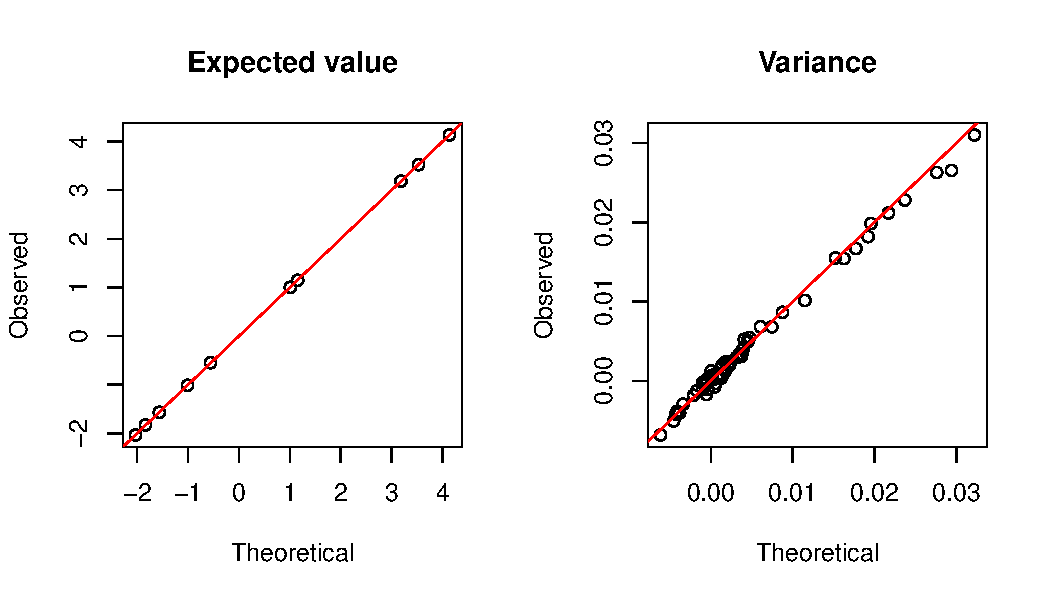
\includegraphics[width=\maxwidth]{figure/q2_graphs-1} \caption[Observed vs]{Observed vs. Theoretical Expectation and Variance for the centered ridge estimator}\label{fig:q2_graphs}
\end{figure}


\end{knitrout}


\section*{Question 3}
See R code in ``ridge\_crossval.R''.

\section*{Question 4}

\section*{Question 5}
\subsection*{(a)}
The objective function can be rewritten as:

\begin{eqnarray*}
  g(\beta,\sigma^2) &=& \frac{n}{2}\log(\sigma^2) + \frac{1}{2\sigma^2}\|\tilde{Y}-\tilde{X}\beta\|^2 + \frac{\lambda}{2}\|\beta\|^2 \\
        &=& \frac{n}{2}\log(\sigma^2) + \frac{1}{2\sigma^2}(\tilde{Y}^\top\tilde{Y}-2\beta^\top\tilde{X}^\top\tilde{Y} + \beta^\top\tilde{X}^\top\tilde{X}\beta) + \frac{\lambda}{2}\beta^\top\beta,
\end{eqnarray*}
then the partials are calculated as:

\begin{eqnarray*}
  \nabla_\beta g(\beta,\sigma^2) &=& \frac{1}{2\sigma^2}\left( -2\tilde{X}^\top\tilde{Y} + 2\tilde{X}^\top\tilde{X}\beta \right) + \lambda\beta
\end{eqnarray*}
\begin{eqnarray*}
  \nabla_{\sigma^2} g(\beta,\sigma^2) &=& \frac{n}{2\sigma^2} - \frac{(\tilde{Y}^\top\tilde{Y} - 2\beta^\top\tilde{X}^\top\tilde{Y} + \beta^\top\tilde{X}^\top\tilde{X}\beta)}{(\sigma^2)^2}.
\end{eqnarray*}

\subsection*{(b)}
The second derivative with respect to $\sigma^2$ is given by:
\begin{eqnarray*}
  \nabla_{\sigma^2}^2 g(\beta,\sigma^2) &=& -\frac{n}{2(\sigma^2)^2} + \frac{2(\tilde{Y}^\top\tilde{Y} - 2\beta^\top\tilde{X}^\top\tilde{Y} + \beta^\top\tilde{X}^\top\tilde{X}\beta)}{(\sigma^2)^3},
\end{eqnarray*}
Since this could be negative, we know that $g$ cannot be convex.

\section*{Question 6}







\end{document}
